\chapter{Introducción}

Deep Learning se enmarca en el área de las Ciencias de la Computación, que es el área de la \emphname{Inteligencia Artificial} (IA).

\section{Inteligencia Artificial antes de Machine Learning}
El área de la IA se enfoca en crear procesos automáticos, que tenga un comportamiento ``inteligentes'', en donde nos referiremos a inteligente (de forma bastante egocéntrica) de que funcione como los humanos. Así mismo, dentro de la IA, se encuentra \emphname{Machine Learning} (ML) (aka Aprendizaje de Máquinas), en dónde algunos dicen que es más bien un área de la estadística. Pero para nuestros efectos, ML se encuentra dentro del área de la IA.

\begin{wrapfigure}{r}{0.35\textwidth}
  \begin{center}
    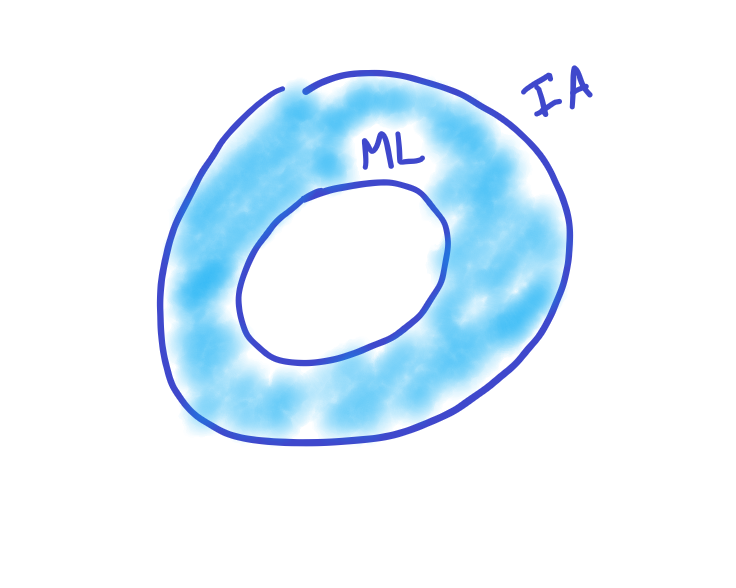
\includegraphics[width=0.3\textwidth]{img/img001.png}
  \end{center}
\end{wrapfigure}

La idea de la IA es que se tienen personas (con mucho dominio) que se juntan para resolver un problema tratando de emular de cómo se puede pensar que lo haría una persona. Lo que se haría usualmente en este caso, es fijarse de una regla que vincule las cosas que están mirando para tratar de emularlo. 

Con esto, la IA se diferencia de ML en que en IA se necesita de mucha ingeniería y de mucho conocimiento experto que está decidiendo de cómo un humano toma decisiones en un algoritmo.

De esta forma, para la IA es muy importante el conocimiento experto: tanto de quien va a generar el proceso como de quién lo programa. 

El cambio de paradigma al introducir ML, es la forma de mirar el problema, pues \textbf{no se va a querer} que un experto decida el cómo una máquina va a resolver el problema, si no que se quiere generar un algoritmo general que, a través de la experiencia, sepa cómo resolver el problema.

\begin{wrapfigure}{l}{0.3\textwidth}
  \begin{center}
    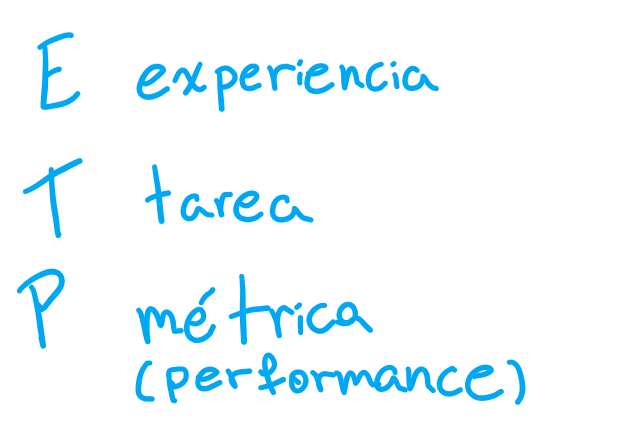
\includegraphics[width=0.25\textwidth]{img/img002.png}
  \end{center}
\end{wrapfigure}

La \emphname[Experiencia]{experiencia}, desde la perspectiva humana, es lo que permite equivocarse y permitir aprender a partir de los errores anteriores. 

La \emphname[Tarea]{tarea} es lo que se quiere resolver específicamente. Por ejemplo, dada una foto, se quiere determinar si hay un gato, o dado un texto, se quiere saber si el texto es positivo o negativo.

Por último, la \emphname[Métrica]{métrica} intenta determinar qué tan bien se está resolviendo el problema o la tarea. Sin embargo, ¿por qué cuando uno piensa en algoritmos usuales la métrica no aparece? porque usualmente evaluamos la efectividad de un modelo a partir de que si hace bien una tarea o no.

Pero cuando se pasa al paradigma de ML, lo que se va a suponer es que el algoritmo puede no estar muy bueno, y la forma de evaluar esto es a través de una métrica. Sin embargo, se tiene la promesa de que, a través de que se consiga más experiencia, el algoritmo desarrollará mejor una tarea.

Es por esto que se llama ``Aprendizaje de Máquinas'', pues es el proceso en que uno le enseña a una máquina a cómo hacer una tarea.

% La experiencia son los datos históricos, la tarea es lo que se quiere hacer y la métrica es para determinar lo ``que tan bien lo está haciendo''. Por lo usual, se quiere un algoritmo ``perfecto'' que no se equivoque, pero cuando se entra en el área de ML, vamos a tener la disposición de que el algoritmo se equivoque, y vamos a evaluar qué tan bien lo hace  a través de la métrica.

% En ML, con más experiencia, la misma tarea lo hará con mejor métrica.

\section{Machine Learning antes del Deep Learning}

Lo que nos convoca, es \emphname[]{Deep Learning} (DL), y este estará un poquito más adentro de ML

\begin{wrapfigure}{r}{0.33\textwidth}
  \begin{center}
    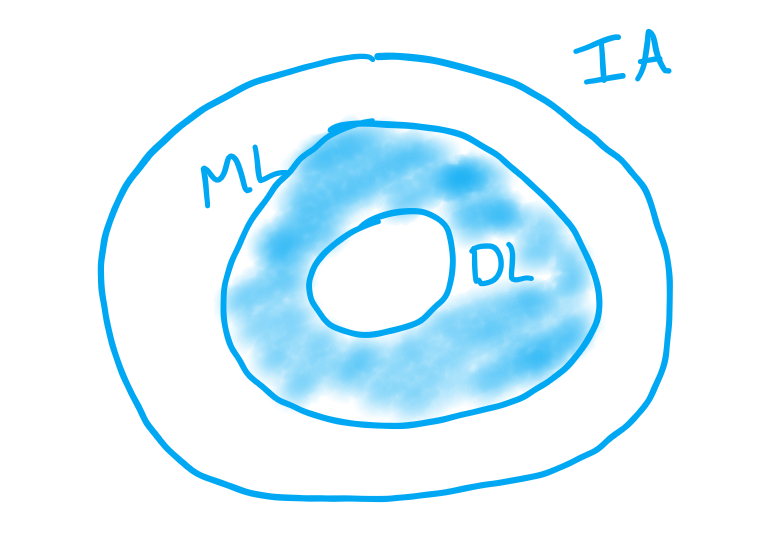
\includegraphics[width=0.3\textwidth]{img/img003.png}
  \end{center}
\end{wrapfigure}

La idea de la diferencia entre ML y DL es la siguiente: en general, los algoritmos de ML se separan en, elegir una tarea, elegir una métrica, y finalmente entregarle experiencia. Y la parte de la experiencia es crucial, pues en nuestro caso, es pasarle \textit{datos}.

Y es importante destacar en cómo hay que pasarle los datos, pues para ML, es crucial pensar en darle datos ``sencillitos'' o ``digeribles'' para el algoritmo. Típicamente se le llama las \emphname[]{características de la entrada}, esto es, la persona tiene que pensar la forma en que se representarán los datos para entregarle a los algoritmos.

Una de las ventajas de esto, es que le simplifica la vida al algoritmo, pues al no pasarle una cantidad enorme de datos, la capacidad de cómputo se ve reducida significativamente.

Y lo segundo, es que un experto en el área puede decidir cuales son los datos relevantes para resolver el problema. Esto se llama \emphname[]{extraer características} antes de pasárselo al computador.

\section{Deep Learning como ``Representation Learning''}

Lo que pasa en DL, es que el cambio de paradigma es bastante radical. La diferencia crucial es evitar precomputar las características de los datos antes de pasárselas al computador. Es decir, se intentará pasar los datos de forma muy ``cruda'' de la información. 

La promesa de DL es que si se le pasa la información muy cruda, ellos aprenderán las componentes principales (o la representación correcta de los datos) de la tarea, \textbf{a la vez que resuelven la propia tarea}. Es más, el nombre más moderno de Deep Learning, está siendo ``Representation Learning'', pues es lo que hace el modelo al fin y al cabo.

así, ya no se necesita decidir a priori cómo representar la experiencia, sino que DL lo hará de forma autónoma.

La forma de representar la experiencia se construirá como una jerarquía. Partiendo desde la información menos abstracta (lo más crudo) hasta lo más abstracta (el resultado), y cuanto más \textit{profundo}, más abstracto se hará la información. Esto justifica el nombre de \textbf{Deep} en Deep Learning. Y lo que ha mostrado la experiencia, es que a medida que se agregan más capas de abstracción exista, mejor será la métrica del algoritmo.

Sin embargo, algunas veces se querrá introducir algún tipo de sesgo para mejorar la métrica del algoritmo, pero de allí dependerá caso a caso.

\section{¿Por qué Deep Learning?}

\begin{wrapfigure}{l}{0.43\textwidth}
  \begin{center}
    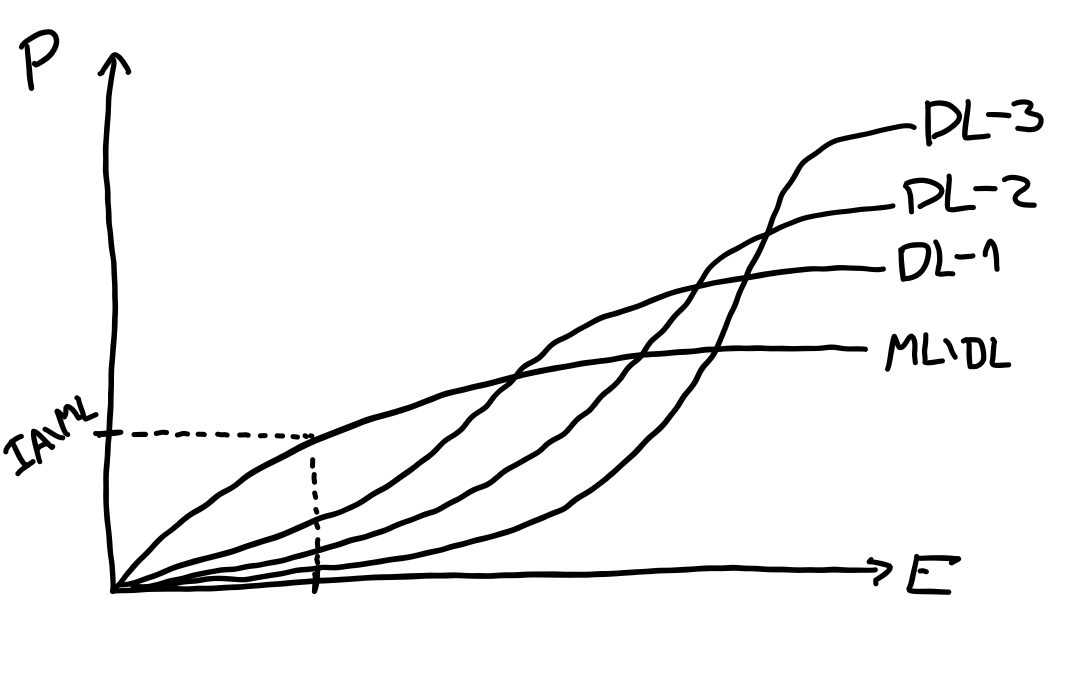
\includegraphics[width=0.4\textwidth]{img/img004.png}
  \end{center}
\end{wrapfigure}

En el gráfico se puede observar la métrica en el eje Y, y la experiencia en el eje X.

En un principio, la IA sin ML se puede ver con un desempeño medio. Se puede ver en el gráfico como IA \textbackslash ML, y que cuando se utilizan los algoritmos de ML (sin incluir los algoritmos de DL) al principio tiene un desempeño mediocre, pues no se le ha pasado suficiente experiencia. Esto sigue así hasta llegar a un límite.

Luego, con DL, se puede observar que a medida que la complejidad crece, el desempeño (la métrica) va creciendo a su vez que la experiencia crece, superando con creces a los algoritmos de ML.









\chapter{Red Neuronal}

\section{El Perceptrón}

Esta corresponde la unidad más básica de una red neuronal. Al principio, el perceptrón fue inspirada en una neurona: una unidad básica del cerebro. El comportamiento de una neurona es, al fin y al cabo, bastante simple; tan simple, que los matemáticos intentaron simularlo para comprobar si se puede obtener pensamiento inteligente. Es así cómo se ``formalizó'' el comportamiento de una neurona de forma matemática, o llevarla a un nivel computacional.
\begin{figure}
\begin{subfigure}{.47\textwidth}
    \centering
    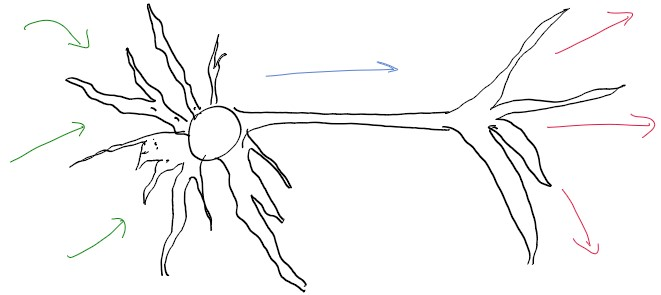
\includegraphics[width=\linewidth]{img/img005_neu_real.jpg}
    \caption{Representación de una neurona ``real''.}
    \label{fig:neu-real}
\end{subfigure}
\begin{subfigure}{.47\textwidth}
    \centering
    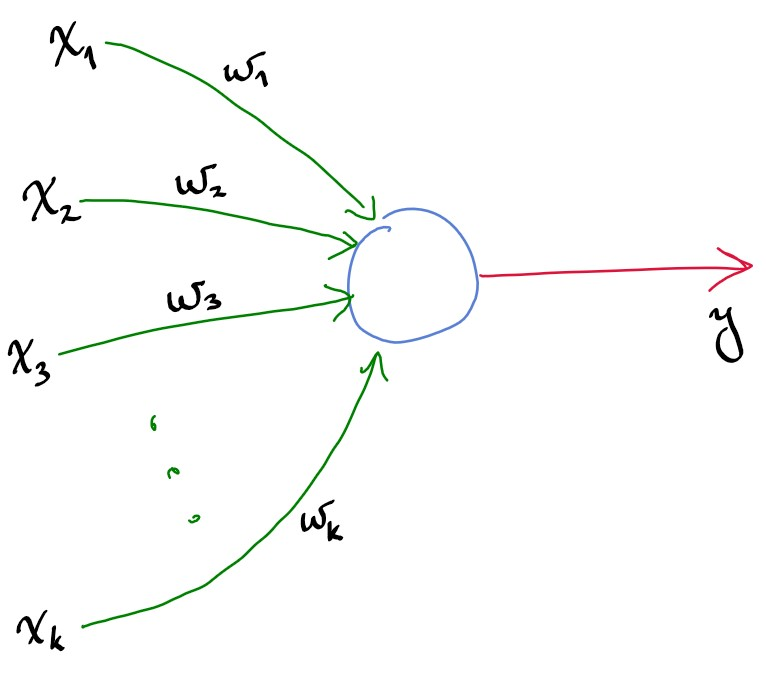
\includegraphics[width=.6\linewidth]{img/img006_neu_falsa.jpg}
    \caption{Representación del Perceptrón.}
    \label{fig:neu-virt}
\end{subfigure}
\end{figure}


\textbf{¿Cómo funciona el Perceptrón?} Tendremos la variable $u$ que representa cuánta información está recibiendo el Perceptrón. Esta variable será la suma de las variables por sus pesos (más un sesgo, a.k.a. bias)
\begin{equation}
    u = x_1 \cdot w_1 + x_2 \cdot w_2 + \ldots + x_k \cdot w_k + b
\end{equation}

Mientras que la salida del perceptrón $y$ será $u$ aplicada en alguna función, llamada \emphname[Función de Activación]{función de activación}
\begin{equation}
    y = f(u)
\end{equation}

\subsection{Funciones de activación}

\begin{figure}
\begin{subfigure}{0.5\textwidth}
    \centering
    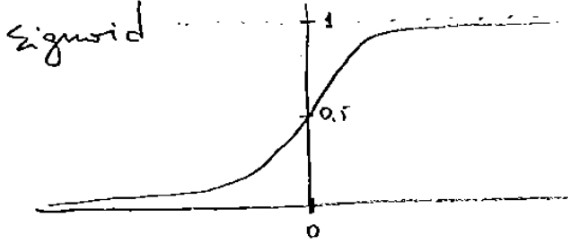
\includegraphics[width=.7\textwidth]{img/img007func_act_sigmoid.jpg}
    \caption{Función de activación Sigmoide}
    \label{fig:sigmoide}
\end{subfigure}
\begin{subfigure}{0.5\textwidth}
    \centering
    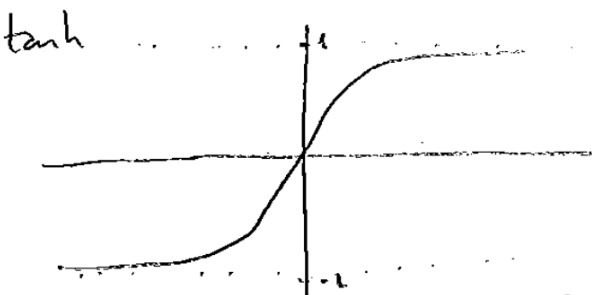
\includegraphics[width=.7\textwidth]{img/img008func_act_tanh.jpg}
    \caption{Función de activación tangente hiperbólica}
    \label{fig:tanh}
\end{subfigure}\\
\begin{subfigure}{0.5\textwidth}
    \centering
    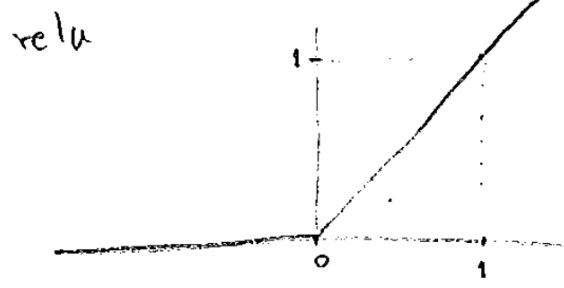
\includegraphics[width=.7\textwidth]{img/img009func_act_relu.jpg}
    \caption{Función de activación ReLU}
    \label{fig:relu}
\end{subfigure}
\begin{subfigure}{0.5\textwidth}
    \centering
    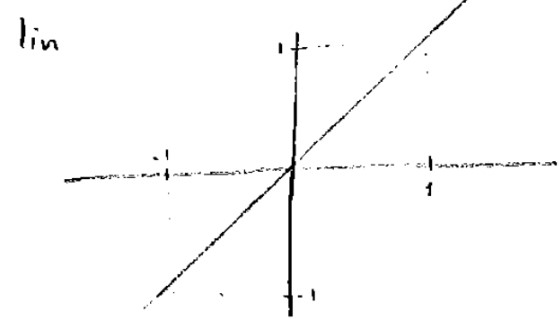
\includegraphics[width=.7\textwidth]{img/img010func_act_lin.jpg}
    \caption{Función de activación Lineal}
    \label{fig:lin}
\end{subfigure}
\caption{Distintas funciones de activación}
\label{fig:act-func}
\end{figure}

A continuación se verán los distintos tipos de funciones de activación que existen:

\subsubsection*{Función escalón}
Es una función que no se ocupará mucho, sin embargo, es la más simple de todas. 
\begin{equation}
    \step(x)=
    \begin{cases}
    1 & \mbox{si } x\geq 0\\
    0 & \mbox{si } x\leq 0
    \end{cases}
\end{equation}

\missingfigure{Función escalón}

\subsubsection*{Función sigmoide}
La idea de la función sigmoide es que es como la función escalón, pero es continua y ``suave''
\begin{equation}
    \sigmoid(x) = \frac{1}{1 + e^{-x}}
\end{equation}

% \begin{figure}
%     \centering
%     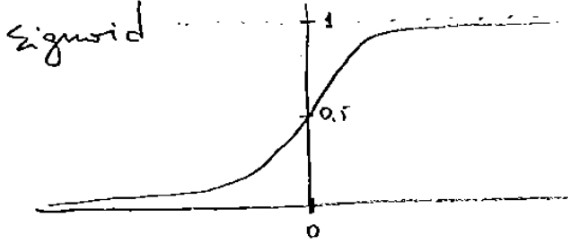
\includegraphics[width=.5\textwidth]{img/img007func_act_sigmoid.jpg}
%     \caption{Función sigmoide}
%     \label{fig:sigmoide}
% \end{figure}

\subsubsection*{Función tangente hiperbólica}
Esta función de activación es cómo el símil de la función sigmoide, solo que en el régimen negativo tiende a -1 en vez de a 0. Esto se interpreta como que el perceptrón ``chupa información'' en los negativos, y ``bota información'' en los positivos.

Por mucho tiempo no se ocupó esta función de activación en los Perceptrones, principalmente porque la gente que trabaja en esta área eran muy puristas, y decían que los Perceptrones deben de parecerse lo más que se pueda a las neuronas.

Veremos más adelante que esta función de activación, en algunos casos, tiene mejor desempeño que la función sigmoide.
\begin{equation}
    \tanh(x) = \frac{e^u - e^{-u}}{e^u + e^{-u}}
\end{equation}

% \begin{figure}
%     \centering
%     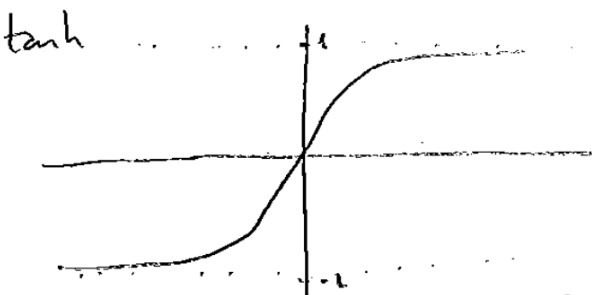
\includegraphics[width=.5\textwidth]{img/img008func_act_tanh.jpg}
%     \caption{Función Tangente Hiperbólica}
%     \label{fig:tanh}
% \end{figure}

\subsubsection*{Función ReLU}

Esta función viene del nombre Rectified Linear Unit.

La definición es bastante sencilla:
\begin{equation}
    \relu(x) = 
    \begin{cases}
        u & \mbox{si } u>0\\
        0 & \mbox{si } u\leq0\\
    \end{cases}
\end{equation}

\subsubsection*{Función lineal}

Esta función es la más sencilla de todas, que es prácticamente la identidad.

\begin{equation}
    \lin(x) = x
\end{equation}

Varios perceptrones:

\missingfigure{Imagen de redes neuronales con capas escondidas}

\begin{example}\namethm{XOR}
Ejemplo XOR

\missingfigure{Tabla del XOR}
\missingfigure{Red del XOR}

\begin{align*}
    h1 &= \relu({x}_1 \cdot 1 + {x}_2 \cdot 1 + 0) & y &= {h}_1 - 2 {h}_2\\
    h2 &= \relu({x}_1 \cdot 1 + {x}_2 \cdot 1 - 1) &  &
\end{align*}

Calculamos cada caso a caso:
\begin{equation*}
\left.
\begin{array}{rclcrcl}
    {x}_1 &=& 0 &\implies& {h}_1 &=& \relu (0+0) = 0 \\
    {x}_2 &=& 0 &\implies& {h}_2 &=& \relu (0+0 - 1) = 0
\end{array}
\right\} \implies y = 0 - 2 \cdot 0 = 0 \quad \checkmark
\end{equation*}
\begin{equation*}
\left.
\begin{array}{rclcrcl}
    {x}_1 &=& 0 &\implies& {h}_1 &=& \relu (0 + 1)     = 1 \\
    {x}_2 &=& 1 &\implies& {h}_2 &=& \relu (0 + 1 - 1) = 0
\end{array}
\right\} \implies y = 1 - 2 \cdot 0 = 1 \quad \checkmark
\end{equation*}
\begin{equation*}
\left.
\begin{array}{rclcrcl}
    {x}_1 &=& 1 &\implies& {h}_1 &=& \relu (1 + 0)     = 1 \\
    {x}_2 &=& 0 &\implies& {h}_2 &=& \relu (1 + 0 - 1) = 0
\end{array}
\right\} \implies y = 1 - 2 \cdot 0 = 1 \quad \checkmark
\end{equation*}
\begin{equation*}
\left.
\begin{array}{rclcrcl}
    {x}_1 &=& 1 &\implies& {h}_1 &=& \relu (1 + 1)     = 2 \\
    {x}_2 &=& 1 &\implies& {h}_2 &=& \relu (1 + 1 - 1) = 1
\end{array}
\right\} \implies y = 2 - 2 \cdot 1 = 0 \quad \checkmark
\end{equation*}

Aquí, la red del perceptrón computa de una forma distinta a como entrenar (?) en computación, no ``manipular símbolos'', si no opero valores.

Podemos escribirlo así:
\begin{align*}
    (h_1 \ h_2) &= \relu\left( 
    (x_1 \ x_2) \spalignmat{1 1; 1 1} + (0 \ -1)
    \right) \\
    (y) &= (h_1 \ h_1) \spalignmat{1;-2}
\end{align*}

Y si introducimos la siguiente notación
\begin{align*}
    \bm{x} &= \spalignmat{x_1 x_2} & W &= \spalignmat{1 1; 1 1} & \bm{b} &= \spalignmat{0 -1} & U &= \spalignmat{1; -2}
\end{align*}

Entonces la forma de generalizar las ecuaciones anteriores es de la siguiente forma:
\begin{align*}
    \bm{u} &= \bm{x} W + \bm{b} \\
    \bm{h} &= \relu(\bm{u}) \\
    y &= \bm{h} U
\end{align*}
\end{example}

Así podemos darle estructura a todo esto:

\missingfigure{Explicacion de la capa de input, escondida y output}







\newpage
\section{}
\FMG{Incluir la definición de Red Neuronal y sus capas}

\missingfigure{Dibujo de la red neuronal}

\FMG{Incluir el ejemplo de XOR}

Al final, dentro del dibujo, lo que más importante es lo que describen las ecuaciones:
\begin{eqnarray}
\bm{h} &=& f(\bm{x} W + \bm{b})\\
y &=& g(\bm{h} U + c)
\end{eqnarray}

Ahora veremos el siguiente teorema:

\begin{theorem}\namethm[UAT]{Teorema de Aproximación Universal}
Sea $F$ una función continua $[0, 1]^k \to [0, 1]$, entonces para todo $\epsilon>0$ existen $W, \bm{b}, U$ tal que $F(x) = \sigmoid(\bm{x}W + \bm{b})U$ se tiene que:
\begin{equation}
    |f(x) - F(x)|< \epsilon \quad \forall x \in [0, 1]^k
\end{equation}

\end{theorem}

Lo importante de este teorema, es que nos garantiza que tan solo basta la estructura de la red neuronal para acercarse a cualquier función continua tanto como uno quiera.

Notemos que el teorema te dice que existen los parámetros, pero no te dicen de qué dimensiones son. Existen estudios que dicen que las cotas son estúpidamente grandes, y que realmente es infactible hacer una única red neuronal ``apilando'' Perceptrones. 

Sin embargo, hay otros estudios que dicen que la efectividad aumenta conforme se van apilando Perceptrones, pero que se necesitan tantos como un crecimiento exponencial, mientras que si se agregan más capas ocultas, se necesitará un orden lineal.

Esto último nos motiva a añadir más capas ocultas, de esta forma:
\missingfigure{Red Neuronal con muchas capas}

Esta forma de red neuronal se llama MLP

La descripción matemática es la siguiente:
\begin{eqnarray}
\bm{h}^{(0)} &=& \bm{x}\\
\bm{h}^{(i)} &=& f^{(i)}(\bm{h}^{(i-1)} W^{(i)} + \bm{b}^{(i)})\\
y &=& g(\bm{h}^{(L)}U + c)
\end{eqnarray}

Y se tienen que calcular estas ecuaciones consecutivamente, haciendo esto, lo llamamos ``\textit{forward}'' (pasada hacia adelante)

\begin{note}
En general usaremos la red para computar una predicción y compararla con el valor real que ya conocemos. En este caso generalmente denotaremos por $\hat{y}=\forward(x)$ para diferenciar ``$\hat{y}$'' de ``$y$'' que usaremos para denotar el valor ``real''.
\end{note}

¿Qué usaremos como función de salida? dependerá mucho de la tarea (y función pérdida que veremos más adelante)

En general queremos \textbf{probabilidades}. Por ejemplo:

\begin{enumerate}
    \item Clasificación binaria:
    \begin{itemize}
        \item Una única neurona
        \item valor de salida entre 0 y 1
        \item Interpretación: Si la respuesta es mayor a 0.5, entonces la respuesta es 1, y en caso contrario, es 0
        
        
    \end{itemize}
    Para este caso, podemos usar una sigmoid como salida
    
    \item Clasificación en varias clases:
    \begin{itemize}
        \item Si tenemos $C$ clases usaremos $C$ neuronas en la caja de salida
        \item Necesitaremos una función que tiene valores
        \begin{equation*}
            (u_1, u_2, u_3,\ldots, u_C)
        \end{equation*}
        
        y me permite interpretarlos como probabilidades
        \item La más usada (más adelante veremos porqué) es ``\textit{softmax}''
    \end{itemize}
    \begin{equation*}
        \softmax(u_1, u_2, u_3,\ldots, u_C) = (s_1, s_2, s_3, \ldots, s_C)
    \end{equation*}
    
    Donde
    \begin{equation*}
        s_i = \frac{e^{u_i}}{\sum_{j=1}^{C}e^{u_j}}
    \end{equation*}
    
    Con esto, tenemos $\sum s_i = 1$ y $0\leq s_i\leq1$. Observemos que softmax amplifica las diferencias en los valores de input. Por ejemplo:
    \begin{align*}
        \softmax(0, 2) &= (0.12, 0.88) &
        \softmax(0, 10) &= (0.00005, 0.99995)
    \end{align*}
    \begin{equation*}
        \softmax(0, 0, 10) = (0.00005, 0.00005m 0.9999)
    \end{equation*}
    
    Así, podemos dar una interpretación:
    \begin{equation*}
        \hy = \softmax(u_1, \ldots, u_C) = (\hy_1, \ldots, \hy_C)
    \end{equation*}
    
    Donde
    \begin{equation*}
        \prob(x\mbox{ pertenece a la clase $i$ según la red neuronal}) = \hy_i
    \end{equation*}
    
    En estos casos los veremos como modelos probabilísticos (parametrizados)
\end{enumerate}

\textbf{Entrenamiento}: Supongamos que tenemos los ejemplos $\conj{(x^{(1)}, y^{(1)}), (x^{(2)}, y^{(2)}), \ldots, (x^{(N)}, y^{(N)})}$. ¿Qué tan bien (o mal) lo está haciendo la red? Supongamos que esperamos un valor $y^{(i)}$ y observamos que la red nos dice que $\hy^{(i)} = \forwardx(x^{(i)})$. Vamos a medir el \textit{error} con alguna métrica, digamos $\error$, así, $\error(\hy^{(i)}, y^{(i)})$ nos indica ``qué tan lejos'' están $y^{(i)}$ y $\hy^{(i)}$. Finalmente, consideraremos el error promedio por medio de
\begin{equation*}
    \L = \frac{1}{N} \sum_{i=1}^{N} \error(\hy^{(i)}, y^{(i)})
\end{equation*}

¿De qué depende $\L$? depende de la red y lo que defina la red: $W\entr[1], b\entr[1], W\entr[2], b\entr[2], \ldots, W\entr[L], b\entr[L], U, c$. Todos estos valores son \textbf{parámetros}, que lo denotaremos por $\theta$, y escribiremos con esto $\L(\theta)$ (es decir, $\L$ depende de $\theta$)

Así, lo que nos gustaría es que $\L$ sea tan pequeño como se pueda, esto nos trae al siguiente problema:

\textbf{Problema}: Encontrar $\hat{\theta}$
que minimiza a $\L(\theta)$. Es decir, tenemos que buscar
$\hat{\theta} 
= \argmin_{\theta} \L(\theta)$

Teniendo $L$ capas, $d$ neuronas en capa escondida, vemos que para computar una red neuronal se necesita $\mathcal{O}(Ld^{2})$. Vemos con un caso concreto cómo crece esto:
\begin{equation*}
    \begin{array}{lcrlcrcl}
    L &=& 10 & d&=&10 &\rightarrow& 1000\\
    L &=& 10 & d&=&100 &\rightarrow& 100000\\
    L &=& 10 & d&=&1000 &\rightarrow& 10000000
    \end{array}
\end{equation*}

Esto quiere decir, que en la mayoría de los casos resultará ``caro'' computar una pasada hacia adelante.

\textbf{Idea}: Si muevo ``un poquito'' uno de los parámetros ¿Cómo cambia la pérdida/error?
\begin{itemize}
    \item Si el error disminuye me conviene
    \item Si el error aumenta no me conviene el cambio
\end{itemize}

Pero como dijimos antes, es muy caro hacer un cambio y (?) $\implies$ lo hacemos (?) (?)

\missingfigure{Figura que muestra el descenso del gradiente}

Obteniendo la derivada $\partial_\theta \L$, ocuparemos el entrenamiendo por descenso del gradiente:
\begin{algorithm}
\tcp{Repetir por $e$ veces}
\For{$\_=1$ \KwTo $e$}{
$\theta_{new} = \theta_{old} - \alpha \partial_{\theta} \L (\theta_{old})$
}
\end{algorithm}

En general lo que tenemos que hacer es (?) en un log, como sigue inicializa $\hat{W}\entr, \hat{b}\entr, \hat{U}, \hat{c}$ de manera aleatoria, decide $\alpha$
\begin{algorithm}
\tcp{Repetir por $e$ veces (o mientras alguna condición de detención no se alcance)}
\For{$\_=1$ \KwTo $e$}{
% $\theta_{new} = \theta_{old} - \alpha \partial_{\theta} \L (\theta_{old})$
$\hat{W}\entr = \hat{W}\entr - \alpha \partial_{W\entr}\L(\hat{\theta}) $\;
$\hat{b}\entr = \hat{b}\entr - \alpha \partial_{b\entr}\L(\hat{\theta}) $\;
$\hat{U}\entr = \hat{U}\entr - \alpha \partial_{U}\L(\hat{\theta}) $\;
$\hat{c}\entr = \hat{c}\entr - \alpha \partial_{c}\L(\hat{\theta}) $\;
}
\end{algorithm}

\section{Back propagation}

Back propagation es simplemente un método para calcular $\nabla_{\theta}\L(\theta)$ y (?) oficialmente en el computador.

Primer concepto importante: Computational graph

\missingfigure{Imagen del Computational graph}

Esto representa una forma de organizar todas las operaciones que englocan la pasada hacia adelante y el cálculo de pérdida.

¿Cómo calculo $\partial_{W_{ij}\entr[2]}\L$?
``simplemente'' calculando lo siguiente:
\begin{equation*}
    \L = \error(g(f\entr[L](f\entr[L-1](\ldots f\entr[2](h\entr[1]W\entr[2] + b\entr[2])W\entr[3] \ldots))))
\end{equation*}

(Okay, no parece una tarea fácil :c) 

Idea: usar agresivamente la regla de la cadena!

Consideremos un conmputational graph simple







\newpage
Clase 10-2020

\section{Generalización}

En general en ML no solo se desea optimización. En DL se desea ajustar los parámetros de forma que el error que se comete sea muy pequeño, pero además, se desea que la red prediga ejemplos que no vio en la fase de entrenamiento.

Entonces no solo interesa disminuir el error, si no que se desea que prediga, y que el error sea bajo. Este concepto se llama \emphname{generalización}. Que el error sea bajo en este conjunto, se le llama el error de generalización.

Esto corresponde al error esperado que la red va a cometer sobre datos nuevos.

En general se necesita una métrica. Esto nos dice qué tn bien lo está haciendo la red. Usualmente, la métrica nos tiene que decir información relevante sobre la red. Típicamente la métrica más estándar es el porcentaje de acierto.

En la práctica, hay que definir la métrica \textbf{pronto} para ir pensando cuál métrica se desea maximizar. Esto dependerá del problema.

Para ir mirando el error de generalización, lo que se hace es conseguirse dos conjuntos de datos.

En la práctica, no se tiene solo un conjunto de entrenamiento, se tienen dos: Train Set (que se utiliza para ajustar los parámetros) y el Test Set (que se utiliza para determinar el error de la generalización).

¿De qué se trata de todo lo que se hace en ML (y en particular en DL)? Se trata de disminuir al máximo el error de entrenamiento en el Train Set, comenzando con parámetros aleatorios de los parámetros. Ahora, si se ajusta los parámetros en el Train Set, resulta natural que el error cometido en el primer conjunto, es siempre menor o igual al del segundo conjunto. Esto siempre debe de ocurrir, por que se está ocupando ese conjunto para entrenar, y la red se ``se sobre ajusta'' a aquel conjunto.

Cuando el Train Error es muy parecido al Test Error, se puede decir que la red es capaz de generalizar. De esta forma, se tienen dos objetivos:
\begin{enumerate}
    \item Disminuir Train Error
    \item Intentar la Diff, Train y Test Error sea chica.
\end{enumerate}

Cuando no se logra disminuir el Train Error, se cometerá \textit{underfitting}, esto significa que mi modelo no tiene la capacidad suficiente para que el error en el train sea bajo. Por otro lado, si no se logra disminuir el Test Error, se cometerá \textit{overfitting}. Esto significa que la diferencia entre el Train Error y el Test Error es muy grande.

Un modelo es como una familia de parámetros. A la hora de hacer una red neuronal, todas las posibles funciones que se pueden crear a partir de esta red. Este conjunto de funciones se llama \textit{capacidad}. Y el entrenamiento se basa en empezar en un ``punto'' dentro de esta capacidad, y lo que se trata de hacer es explorar toda la capacidad hasta encontrar la función que mejor se ajusta a los datos.

Uno jamás tiene que ocupar el conjunto de test para decidir algo sobre el modelo. Solo debe de ser ocupado para evaluar como se comportará el modelo con datos que no ha visto nunca. La cantidad de capa y el número de neuronas gobierna en la capacidad de la red, pues ayuda a alcanzar más posibles funciones. En general, todos los parámetros que gobiernan la capacidad del modelo se llaman hiperparámetros. Esto es porque son cosas que se pueden manejar y variar. 

En general, cuanta más capacidad se tiene, menos error se obtiene. Así, no se puede ocupar el Train Set para determinar la capacidad correcta (en este caso, la combinación de de capas y neuronas), es de aquí en donde nace el \textit{Dev Set} (Conjunto de desarrollo, Development) también se llama conjunto de validación en el contexto general de ML.

El conjunto de Test se deja a un lado, y no se piensa en ocupar jamás para calibrar parámetros. El conjunto de Train se utilizará para ajustar los parámetros, y el conjunto de Dev se utilizará para buscar una capacidad correcta. Esto significa que se miran ambos conjuntos (Train y Dev) para mirar que tan bien o mal está. 

En general, una de las recetas es generalmente la siguiente:
\begin{enumerate}
    \item Primero hay que intentar en disminuir el Train Error (esto es, evitar el underfitting). Esto significa que hay que aumentar capacidad hasta llegar un trade off razonable, y cuando se llega a este límite, allí recién se empieza a ver la diferencia entre train y dev.
    \item Un momento cuando se sabe que no hay underfitting, se empieza a revisar el test set. Si es que no existe overfitting, el problema se acabó. 
    \item Si es que existe el overfitting (es decir, la diferencia entre train error y test error es alta) hay que cambiar un hiperparámetro que \textbf{no cambie la capacidad}. Porque si es que se aumenta la capacidad, entonces se seguirá aumentando la brecha entre ambos. Típicamente lo que se hace es acortar capacidad, aunque lo que se hace hoy en día es la regularización. 
    
    Típicamente los hiperparámetros que no aumentan capacidad, es el número de ejemplos (más ejemplos no aumenta capacidad) o bien disminuir el número de capas, o aplicar regularización. Y luego, se empieza en el paso 1. de nuevo.
\end{enumerate}

La forma de dividir estos conjuntos, típicamente en ML se utiliza $60 / 20 / 20\%$. Pero en DL, para entrenar redes neuronales, típicamente se utilizan muchísimos ejemplos, digamos, 10 millones. ¿Tiene sentido utilizar 2 millones de ejemplos para el conjunto de test? No. Bastarían 100 mil ejemplos. De hecho, en DL se llegan a casos tan extremos como una proporción del $98 / 1 / 1\%$. Esto nos dice de no asumir este ``'estándar', y ocupar las proporciones de forma que sean cómodas. Además, como el Test set se utiliza para estimar el error de generalización, hay que intentar que su distribución sean lo más parecido a la realidad posible. 




\chapter{Regularización y Optimización}

\section{Regularización}

Regularización son cualquier método que están hechos para disminuir el error de generalización sin aumentar el error de entrenamiento. En palabras más técnicas, se quiere disminuir el error de generalización sin cambiar la capacidad del modelo. Usualmente, lo que hacen los métodos de regularización, es tomar la capacidad del modelo, y darle preferencias unas sobre otras. Es como ``empujar'' las preferencias artificialmente.

\subsection{Regularización a través de \textit{penalty}}
Típicamente, se querrá dar prioridad a funciones más ``simples''. Esto está motivado por lo siguiente: ``si tenemos dos explicaciones para un mismo fenómeno, entonces me quiero quedar con aquel que tenga menos supocisiones''. Esta idea llevada a ML, es que si se tienen dos funciones que tienen el mismo error de entrenamiento, entonces nos queremos quedar con la más ``simple''. 

Esto se puede lograr dando ciertas restricciones a los parámetros que se van a aceptar como válidos. La forma más estándar es por medio de la penalización del tamaño de parámetros. La idea es tratar de empujar el modelo a que aprenda (o que termine con una solución) en donde los valores de los parámetros sean tan pequeños como se pueda.

Si es que se tiene dos redes que tienen el mismo error de entrenamiento, entonces se quiere elegir la que tiene los parámetros más chiquitos, y la forma de hacer esto es teniendo una función que mida que tan grandes son los parámetros y esta función se llama la función de penalización.

Una forma muy simple y elegante de hacerlo, es cambiando la función de error. Por ejemplo, típicamente se escribe así:
\begin{equation*}
    \L' = \frac{1}{N} \sum_{i=1}^N \error(\hy^{(i)}, y^{(i)}) + \alpha  \penalt(\theta)
\end{equation*}

$\penalt$ es una función que dice que tan grande son los parámetros. Así, con esta nueva función de error nos dice el error de las muestras, con una penalización sobre los parámetros. Entonces si la penalización es alta, el error es alto y viceversa.

La gracia es que se puede ocupar el mismo algoritmo de Backpropagation para optimizar. Pero es importante notar que no cambia la capacidad de la red. Lo que dices es que si el argumento es alto, entonces se penalizará.

Todo lo que importa ahora es la función $\penalt$. La más estándar es la llamada $\ell_2$. Esta se define como sigue: suponiendo que $\theta = (W^{(1)}, b^{(1)}, \ldots, U, c)$, entonces
\begin{equation*}
    \penalt-\ell_2(\theta) = \frac{1}{2} \left(
    \norm{W^{(1)}}_2 + \ldots \norm{U}_2
    \right)
\end{equation*}

Donde $\norm{A}_2 = sum(A \ast A)$. OJO: No se están considerando los bias (existe un motivo importante para esto).

\subsection{Regularización por \textit{weight decay}}

Algo que se puede decir es: pero si ya hicimos todas las derivadas con $\L$, ¿ahora habrá que rehacer todas las derivadas para $\L'$? La gracia es que, como pusimos una suma en $\L'$, entonces la derivada de la suma sera la suma de las derivadas, simplificando enormemente el cálculo de ésta.

En efecto, hagamos la derivada para una de las componentes
\begin{eqnarray*}
\frac{\partial \L'}{\partial W^{(k)}_{ij}}
= \frac{\partial \L}{\partial W^{(k)}_{ij}} + \frac{\alpha}{N} W^{(k)}_{ij}
\end{eqnarray*}

¿Por qué se hace todo esto? porque en general las librerías cuando se quiere hacer penalización $\ell_2$, no se hace en la Loss, por la siguiente razón:

cuando ahora se haga un paso del descenso del gradiente, se vería así:
\begin{eqnarray*}
W^{(k)}_{ij} &:=& W^{(k)}_{ij} - \lambda \frac{\partial \L'}{\partial W^{(k)}_{ij}}\\
&=&  W^{(k)}_{ij} - \lambda \frac{\partial \L}{\partial W^{(k)}_{ij}} - \frac{\alpha \lambda}{N} W^{(k)}_{ij} \\
&=&  (1 - \beta) W^{(k)}_{ij} - \lambda \frac{\partial \L}{\partial W^{(k)}_{ij}}
\end{eqnarray*}

Donde $\beta = {\alpha \lambda}/{N}$. La fórmula anterior se puede interpretar como que se está parando en un punto, un poco más pequeño que el punto original $W^{(k)}_{ij}$ y de allí se hará descenso del gradiente. El efecto de este paso, es que independiente de a donde se mueva la derivada, siempre se tratará de hacer que el parámetro sea un poco más pequeño (a pesar de que la derivada lo intenta hacer aumentar).

es por esto que usualmente, las librerías ocupan el penalty dentro del descenso del gradiente, donde la función de Loss se sigue manteniendo como el cross entropy. Es por esto que esta regularización se le llama ``\textit{weight-decay}''.

\subsection{Regularización por \textit{Data argumentation}}

Una buena forma de regularización es el ``Data argumentation''. Si uno puede buscar más datos, siempre dará buenos resultados, pero sino se está cambiando la capacidad, posiblemente el training rate suba un poquito. 

Data argumentation consiste en no gastar más plata buscando datasets, si no que del mismo dataset, obtener más muestras de una forma ingeniosa. 

Por ejemplo, si tengo la imagen de un gato, con solo ``voltarla'' (hacer que rote en un eje central) el dataset aumenta al doble. Otras cosas que se hacen es que se cortan un poquito las imágenes.

Una técnica, es hacer que cuando se pida algún dato al dataset, éste busque la información, pero antes de entregarlo, lo modifica un poco antes de entregarlo, de esta forma, podríamos tener un ``dataset infinito''.

Es importante que para esto, hay que ingeniárselas para poder aplicar esta técnica. Esto no siempre es fácil, y hay que ser muy creativo para crear datos donde no los haya. Y más que nada, hay que usarlo cada vez que se pueda ocupar.

\subsection{Regularización por Agrupación}

Otra de las técnicas de regularización, se llama el de Agrupación o ensamblado. Esto está motivado por el siguiente ejemplo: Si es que a mi me duele algo, el doctor dará un diagnostico de esto. Si uno no tiene mucha confianza, entonces se va a preguntarle a otro doctor. Lo que se está suponiendo es que si tenemos a dos doctores, se asume que los dos tienen opiniones diferentes.

Si nos vamos en el caso del DL, los doctores se asemejan a los modelos, donde aquí, se le va preguntando a varios modelos la predicción. Y así para aumentar la confianza en la predicción, en vez de preguntarle a un único modelo, se le pregunte a varios modelos. Lo más estándar es hacerlo por medio de ``votación''.

Si los modelos son independientes, en promedio, se disminuirá el error. Y en general, las competencias de ML o DL las ganan aquellos que tienen varios modelos y promediando los resultados de los modelos. Es más, se le pueden dar distintos pesos a cada modelo, y entrenar estos pesos. Lo anteriormente descrito se llama ``staching''.

\missingfigure{Imagen del minuto \href{https://youtu.be/4cJlTns7noE?t=418}{6:58 de la clase 11}}

\subsection{Regularización por \textit{Bootstrap}}

El último método de regularización es ``Bootstrap''. Esto consiste en lo siguiente: se toma un modelo con sus parámetros. Lo que hace es que en vez de entrenar distintos modelos, lo que se hace es que se entrena el mismo modelo pero con datos distintos.

Veamos esto con un ejemplo. Supongamos que tenemos un conjunto de entrenamiento de tamaño $100$, y que generaremos 5 grupos nuevos de entrenamiento. Estos conjuntos se armaran seleccionando elementos aleatorios del conjunto original, \textbf{pero con reemplazo}. De esta forma, casi seguramente los conjuntos armados tendrán elementos repetidos, y con cada uno de estos conjuntos, se entrenará el mismo modelo. Y finalmente, se puede hacer la misma idea anterior para crear nuevos modelos.

\subsection{Regularización por \textit{Dropout}}

\subsubsection{Introducción}

Supongamos que tenemos un modelo, y que a la hora de entrenar, el modelo se empiece a fijar en algunas características particulares del input para realizar una predicción. Es decir, que de las 100 componentes que pueda tener un vector de entrada, solo se fija en 10 componentes particulares. Esto también puede suceder en las capas ocultas de la red.

\missingfigure{Imagen del minuto \href{https://youtu.be/4cJlTns7noE?t=1111}{18:31 de la clase 11}}

Esto es perjudicial, pues si tenemos --por ejemplo-- una red neuronal que determina si existe una cara en una foto, puede que la red neuronal se sobre ajuste a determinar que hay una cara solo sí hay una nariz en la foto. Esto resulta perjudicial, pues si ahora le pasamos una imagen de alguien tapándose la nariz, o la foto de un payaso a esta red, determinará que no hay ninguna cara en la imagen.

La forma de solucionar esto, es ``desactivando'' algunas neuronas de forma aleatoria antes de pasar el Batch de entrenamiento, y se entrena la red suponiendo que estas neuronas no existiesen. Luego, cuando se le entregue otro Batch, se desactivaran \textbf{otras} neuronas, y se repite el proceso.

El efecto de realizar esto, es que se le está obligando a la red a que no se enfoque en unas pocas neuronas para determinar la predicción. Lo que se desea, es que la red sea capaz de predecir aún cuando le falten neuronas. 

Una analogía es que se le está haciendo el trabajo más difícil a la red, como que si una persona estuviese entrenando para una competencia, en vez de hacer lagartijas con ambos brazos, lo haga primero con uno, y luego con otro. De esta forma, la persona tendrá los dos brazos aún más fuertes que si se le hubiese entrenado con los dos brazos simultáneamente, de forma que estará aún más preparado para la competencia.

\subsubsection{Formalización matemática}

Para aterrizar los conceptos, lo que se hace es elegir alguna capa $i$ y lo que se hace es elegir una ``máscara'' con cierta probabilidad $P_i \in [0, 1]$, y se multiplica punto a punto la salida de la red con la máscara $M_i$. Es decir
\begin{equation}
    h\entr = f\entr(h\entr[i-1] W\entr + d\entr) \ast M_i.
\end{equation}

Otro tema importante es preguntarse cuál probabilidad ocupar. Es necesario notar que el Dropout que se utiliza hoy en día es bien agresivo, en dónde la probabilidad es del $0.5$. A pesar de que suena ``extremo'', realmente funciona muy bien! Así que en general, en las capas finales usualmente se desactivan pocas neuronas, mientras que en el inicio se desactivan bastantes. Sin embargo, no existe una ``buena regla'' de cuántas neuronas desactivar. La gracia de tener probabilidades altas, es que se pueden tener neuronas muy grandes y de esta forma ocupar probabilidades muy agresivas.

Ahora bien, supongamos que en una capa se han desactivado la mitad de las neuronas. En la fase de entrenamiento, por lo usual, las neuronas que reciben la información están esperando un cierto valor, pero cuando se quite el Dropout, las neuronas recibirán \textbf{el doble} de lo esperado. Esto se puede arreglar, ponderando por la mitad (o por la probabilidad $P_i$ ocupada) en todas las neuronas en la capa que se realizó Dropout. De esta forma, las neuronas de la capa siguiente ``percibirán'' en promedio lo que se esperaba.

Sin embargo, lo que se utiliza realmente para solucionar este problema, es el ``Inverted Dropout''. Este consiste en que, momento seguido en que se apagan las neuronas, se amplificará su valor antes de seguir a la siguiente capa. De esta forma, la fórmula final quedaría como
\begin{equation}
    h\entr = f\entr(h\entr[i-1] W\entr + d\entr) \ast \frac{M_i}{P_i}.
\end{equation}

Así que, lo importante a tener en cuenta aquí, es \textbf{que hay que desactivar manualmente el Dropout para ocuparlo}

\subsection{Regularización por \textit{Early Stopping}}

La última técnica de regularización, consiste en \textit{Early Stopping}. Típicamente, la curva de aprendizaje se visualiza así:
\missingfigure{Imagen del minuto \href{https://youtu.be/4cJlTns7noE?t=3050}{50:50 de la clase 11}}

Entonces, hay que notar que no se le esta agregando capacidad, a pesar de que, cuanto más tiempo se deja corriendo la red para entrenar, entonces se está permitiendo que la red llegue a más funciones a las que ajustarse.

El tema es que cuánto más tiempo se deje la red entrenando, éste irá disminuyendo aún más su loss function. Sin embargo, esto no ocurre con la loss function para el Dev set, pues éste irá bajando hasta llegar a un mínimo, y después su loss function empezará a subir. Esto resulta perjudicial, pues es un indicador de que la red se está sobre ajustando.
\missingfigure{Imagen del minuto \href{https://youtu.be/4cJlTns7noE?t=3119}{51:59 de la clase 11}}

Así que la solución a este problema, es que nosotros detendremos a mano el entrenamiento de la red cuando ocurra esto, de forma que ésta tenga un mejor desempeño en un punto en específico. Esto se hará de forma que, cada cierto tiempo, se irá midiendo cómo varía el loss function del Dev set con respecto a train set, y dado algún criterio, se detienen las fases de entrenamiento.

Sin embargo, tiene un problema. Es que se tiene acoplada la idea de disminuir el error de entrenamiento con el error de desarrollo o de generalización. 

\section{Optimización}
% https://youtu.be/4cJlTns7noE?t=3564

Actualmente, nos hemos enfocado en la arquitectura, mientras que a la hora de hacer optimización, no nos hemos enfocado mucho en este tema. Preguntas como ¿Dónde nos paramos inicialmente? En general, no hay mucha teoría en esto, pero hay heurísticas.

Hay varias técnicas que permiten ubicarse en un buen punto, y empezar a bajar de la mejor manera posible.

Supongamos que tenemos varias capas, y que vamos a seguir el camino de algunas conexiones (pesos) $\{w_i\}_{i=1}^{L}$ y $\{h_i\}_{i=0}^{L}$.
\missingfigure{Imagen del minuto \href{https://youtu.be/4cJlTns7noE?t=3745}{1:02:25 de la clase 11}}

Entonces, calculemos la siguiente cantidad:
\begin{eqnarray}\label{eq:dL_dw1}
\frac{\partial \L}{\partial w_1}
&=& \frac{\partial \L}{\partial h_L}
\cdot \frac{\partial h_L}{\partial h_{L-1}}
\cdot \ldots \cdot \frac{\partial h_i}{\partial h_{i-1}}
\cdot \ldots \cdot \frac{\partial h_1}{\partial w_1}
\end{eqnarray}

Calculemos $\frac{\partial h_i}{\partial h_{i-1}}$ explícitamente. Sabemos que
\begin{eqnarray*}
    h_i &=& f(h_{i-1} w_i + \ldots) 
\end{eqnarray*}

Entonces, definiendo como $u_i = h_{i-1} w_i + \ldots$, tendremos que
\begin{eqnarray*}
    \frac{\partial h_i}{\partial h_{i-1}} 
    &=& f'(u_i) w_i
\end{eqnarray*}

Luego, reemplazando esto en la Ec.~\eqref{eq:dL_dw1} tendremos que
\begin{eqnarray}
\frac{\partial \L}{\partial w_1}
&=& \frac{\partial \L}{\partial h_L}
\cdot \prod_{i=1}^{L} f'(u_i) \prod_{i=2}^{L} w_i
\cdot x
\end{eqnarray}

De aquí, si es que uno de estos valores es 0, entonces toda esta multiplicación será $0$ inmediatamente. Por ejemplo, si es que algún $w_i$ es $0$, entonces la derivada será 0.

Observemos además, que si $f$ es una sigmoid, tendremos que su derivada está acotada por $1/4$. De aquí, la expresión $\prod_{i=1}^{L}f'(u_i)$ estará acotado por $(1/4)^{L}$, así que si $L$ es grande, esta cantidad será muy pequeña. Además, si es que se piensa compensar este decrecimiento haciendo aumentar $w_i$, realmente no serviría de mucho, pues $f'(u_i) \approx 0$ cuando $w_i$ es muy grande. Esto nos indica que tendremos que tomar valores de $w_i$ muy cercanos a $0$.

Lo que sucede aquí, es que si se tienen muchas capas, es difícil que el gradiente fluya a las capas principales, pues estas se acercarán cada vez más a $0$. 

Y un problema que existe también, es que no existe buena teoría para decidir dónde partir la optimización, sin embargo, existen algunos consejos para inicializar los parámetros. Por ejemplo, se sugiere que se inicialicen estos parámetros de forma aleatoria, y que sean muy cercanos a $0$.

\subsection{Inicialización de Xavier}

Es más, si se recuerda un poco de estadística, es que que si se empieza a sumar los valores inicializados aleatoriamente, a pesar de que esta suma seguirá centrado en 0, la varianza empezará a aumentar mucho. Entonces lo que se suele hacer, es ponderar el valor inicializado por la cantidad de neuronas existentes en esa capa, de forma que la varianza de la suma no aumente. Es decir, lo que se hace es inicializar los valores de la siguiente forma
\begin{equation*}
    \mathcal{N}(0, 1) \cdot \frac{1}{\sqrt{d_i}}
\end{equation*}

En código, se vería más o menos así
\begin{equation*}
    W\entr = \text{\texttt{randn}}(d_{i-1}, d_i) \cdot \frac{1}{\sqrt{d_{i-1}}}
\end{equation*}

De hecho, esta inicialización tiene un nombre, y se llama Xavier.

\subsection{Inicialización de He}

Lo segundo, es que existe otra ``innovación'', es que si se ocupa la función de activación $\relu$, entonces conviene inicializar los valores de la siguiente forma
\begin{equation*}
    W\entr = \text{\texttt{randn}}(d_{i-1}, d_i) \cdot \sqrt{\frac{2}{d_{i-1}}}
\end{equation*}

Esta multiplicación de $\sqrt{2}$ se debe a que la derivada de $\relu$ no es simétrica, como lo es el sigmoid o la tangente hiperbólica. Entonces la media estará más ``empujada'' a la derecha. Esta inicialización se llama la inicialización de He.

Lo que se gana con esto, es que es más estable en el aprendizaje.

\subsection{Inicialización por medio de una uniforme}

Otra de las cosas, es que en vez de inicializar los valores a través de una normal, se puede incializar a través de una uniforme. Sin embargo, en este caso se modifica un poco la constante de ponderación
\begin{equation*}
    W\entr = \text{\texttt{uniform}}\left(-\sqrt{\frac{6}{d_{i-1}}}, \sqrt{\frac{6}{d_{i-1}}}\right)
\end{equation*}

La razón de esto es un poco similar a lo explicado anteriormente. Es que si se calcula la varianza de una uniforme entre -1 y 1, resulta ser $1/6$. Entonces para compensar un poco esto, hay que multiplicarlo por $\sqrt{6}$, y de esta forma asegurarse que la varianza se mantenga estable.

No se puede dar muchos más detalles al respecto, pues son simplemente heurísticas, es decir, solo hacen que todo ``funcionen bien''. Y con esto, dada una buena inicialización, hará que uno se siente más seguro de que se puede añadir una capa más a la red y no va a ser más inestable el aprendizaje.

\subsection{Normalización del Input}

Otra cosa que se quiere hacer es \textbf{normalizar el input}. ¿A qué se refiere con esto? supongamos que tenemos el siguiente conjunto de datos:
\begin{equation*}
    \mathcal{D} = \conj{(x\entr[1], y\entr[1]), \ldots, (x\entr[n], y\entr[n])}
\end{equation*}

En general, a uno no le gustaría que las características, por tener más o menos escala, signifiquen más o menos para la red. Por ejemplo, si tuviéramos un vector de características donde una de las componentes es la temperatura, la edad, el salario, etc. Todos estos valores tienen escalas distintas, y si se pasan estos datos a la red ``en bruto'', sesgarían a la red. Así que lo ideal es que estos datos estén cercanos al 0 para que ojalá no se empuje a una neurona en particular, por tener la escala diferente.

Lo que hacemos en este caso es normalizar, y esto es bastante simple, sería aplicar la siguiente fórmula. Suponiendo que $X \in \mathbb{R}^{N \times F}$, entonces
\begin{eqnarray*}
    \mu &:=& \frac{1}{N} sum_1(X)\\
    X &:=& X - \mu \\
    v &:=& \frac{1}{N} sum_1 (X \ast X)\\
    X &:=& X / \sqrt{v}
\end{eqnarray*}

Usualmente normalizar es algo ``gratis'', pues no corresponde nada a entrenar, sólo se está trabajando un poco los datos. Además, es ideal hacer esto \textbf{siempre}. 

Algo importante en este sentido, es que si ocupamos un nuevo dato, entonces habrá que restarle la media $\mu$ y dividir por la raíz de la varianza $v$ (¡importante no recalcularlos! sólo la media y la varianza obtenidos de los datos de entrenamiento). Además, es que este proceso sólo se debe hacer \textbf{con los datos de entrenamiento} (¡los datos de test no se toca!). 

\subsection{Batch Normalization}

Supongamos que tenemos una red con varias capas. Observemos que, a pesar de que podemos normalizar los inputs, aún en las capas intermedias, no sabemos que puede ocurrir en las capas ocultas, donde usualmente aquí los valores pueden oscilar mucho. Así que la solución a este problema es lo que se llama como \textit{Batch Normalization}.

Este consiste en, cuando se le entregue un Batch a la red, cuando se encuentre con una de las capas ocultas, se tendrá un ``set'' de neuronas en esa capa (es como una matriz) y la idea es normalizar toda la dimensión con respecto a este Batch. Y lo que se hace realmente es adjuntar ``al lado'' de la capa oculta otra capa llamada Batch Normalization (BN). De esta forma, a la siguiente capa no entra la salida de la capa oculta original, si no que entrarán los datos \textbf{normalizados} de la capa anterior.

\missingfigure{Imagen del minuto \href{https://youtu.be/izOwC2my1Kw?t=2219}{36:59 de la clase 12}}

Esto se puede hacer de la siguiente forma: Escribamos la fórmula de una capa $i+1$
\begin{eqnarray}
h\entr[i+1] = f(h\entr W\entr[i+1] + b\entr[i+1])
\end{eqnarray}

Observemos que $h\entr$ tiene dimensiones de $(B, d_i)$, entonces lo que se hace es calcular las siguientes cantidades
\begin{eqnarray}
\mu\entr &:=& \frac{1}{B} \mbox{sum}_{\dim(1)} (h\entr)\\
v\entr &:=& \frac{1}{B} \mbox{sum}_{\dim(1)} ((h\entr - \mu\entr) \ast (h\entr - \mu\entr))
\end{eqnarray}

Luego calculamos la siguiente cantidad
\begin{eqnarray}
\Tilde{h}\entr := \frac{h\entr - \mu\entr}{\sqrt{v\entr + \epsilon}}
\end{eqnarray}

Con $\epsilon$ pequeño (por si $v\entr$ quedó muy pequeño). Esta última operación es cómo agregarle una ``capa'' nueva. Entonces, a $h\entr[i+1]$ se le pasará $\Tilde{h}\entr$ de la siguiente forma
\begin{eqnarray}
h\entr[i+1] = f(\Tilde{h}\entr W\entr[i+1] + b\entr[i+1])
\end{eqnarray}

Hay que notar que el Batch normalization \textbf{necesita} tener una especia de memoria, pues en la fase de entrenamiento siempre se estuvo ocupando este tipo de normalización, y cuando se introduzca un nuevo dato, no tendrá con quién normalizarse. Existe una forma elegante de esta idea de ``memoria''.

Notemos que esta idea igual es como un poco rara, pues se está \textit{imponiendo} que la red aprenda de esta forma, donde Batch Normalization no tiene ningún parámetro a aprender. Lo que se ha visto que es razonable es lo siguiente: Permitirle a la red de \textbf{no ocupar la capa}, de forma ésta elija si ocuparla o no, pero dejarle que \textbf{ella misma decida}. ¿Cómo se puede implementar esto? Se puede hacer a través de la siguiente ecuación
\begin{eqnarray}
\hat{h}\entr = \gamma\entr \ast \Tilde{h}\entr + \beta\entr
\end{eqnarray}

Dónde $\gamma\entr$ y $\beta\entr$ son parámetros que la red aprenderá. La idea es que a través de $\gamma\entr$ la red regulará la desviación estándar $\sqrt{v\entr + \epsilon}$ y a través de $\beta\entr$ la red regulará el centro $\mu\entr$. Esta es como una capa ``reversible''. Y se pueden inicializar con 1's y 0's, en dónde estos parámetros sí hay que propagarlos con Back-Propagation.

La gracia de esto es que se está \textbf{ayudando a la optimización}, llegando a un óptimo mucho más rápido.

Observemos que $\gamma\entr$ y $\beta\entr$ son parámetros, es decir, serán aprendidos. Pero $\mu\entr$ y $v\entr$ hay que guardarlos \textbf{para cada capa}, es decir, de alguna forma tiene que recordarlas. Alguna de la formas sería ocupar el último, o promediar todos, pero esto tiene el problema de que son muy ``extremas'', así que la solución a esto es el \textbf{promedio móvil exponencial}. La idea de esto es promediar todo, pero dando más pesos a los últimos valores. Esto se realiza de la siguiente forma: 

dropeando el $\entr$ en el $\mu$ y $v$, lo que se hará es actualizar los siguientes valores
\begin{align}
\overline{\mu} &:= \delta \overline{\mu} + (1-\delta) \mu & \overline{\mu} &:= 0 \\
\overline{v} &:= \delta \overline{v} + (1-\delta) v & \overline{v} &:= 0
\end{align}

Esta última expresión se le llama promedio móvil exponencial. Un valor razonable para $\delta$ corresponde a $\delta=0.9$, que esto corresponde promediar a los ``últimos 10''.

\section{Algoritmos de Optimización}

Observemos que los ejemplos hasta aquí han sido en 1D, pero en DL lo usual es que la optimización sea en muchas dimensiones. Supongamos que tenemos una situación como la de la imagen. ¿Qué es lo que pasa si hacemos descenso del gradiente cómo siempre? Lo más probable es que tenga mucha turbulencia al bajar, a pesar de que sabemos que existe una forma óptima de hacerlo
\missingfigure{Imagen del minuto \href{https://youtu.be/izOwC2my1Kw?t=4468}{1:14:28 de la clase 12}}

\subsection{SGD con Momentum}

Lo que nos gustaría es que, en vez de que oscile tanto la optimización, lo que se hará es mirar la oscilación del gradiente y promediar los gradientes anteriores en una dimensión, cómo se observa en la imagen
\missingfigure{Imagen del minuto \href{https://youtu.be/izOwC2my1Kw?t=4535}{1:15:35 de la clase 12}}

Esto se llama \textit{descenso del gradiente con momentum}, es decir, en vez de bajar por el gradiente, se baja por el promedio histórico del gradiente. ¿Cuánto se promedio? se utilizará el promedio móvil exponencial. Esto mejora demasiado el tiempo de convergencia. La forma de realizar esto es a través de aplicar esta fórmula
\begin{eqnarray}
\overline{\partial W} &:=& \beta \overline{\partial W} + (1-\beta) \frac{\partial \L}{\partial W} \\
W &:=& W - \lambda \overline{\partial W}
\end{eqnarray}

Y si definimos $V_{\partial W} = -\lambda \overline{\partial W}$ entonces las ecuaciones anteriores se pueden reescribir como
\begin{eqnarray}
V_{\partial W}
&:=& \beta V_{\partial W} - \lambda' \frac{\partial \L}{\partial W} \\
W &:=& W + V_{\partial W}
\end{eqnarray}

Dónde $\lambda' = \lambda(1-\beta)$ (pero como $\lambda$ es un hiperparámetro que se maneja ``a mano'', la utilización de esta notación no afecta en nada). Esta reformulación se llama \textit{SGD con momentum}. El $\beta$ que aparece en la última ecuación, hace el efecto de disminuir la velocidad del gradiente, en física lo llaman como \textit{el coeficiente de fricción viscoso} y $\lambda$ se le llama como tasa de aprendizaje.

\subsection{SGD con Momentum de Nesterov}

Hay además una pequeña variante a este algoritmo, llamado \textit{SGD + momentum + Nesterov}. Este método se implementa como sigue
\begin{align*}
    \Tilde{W} &:= W + \beta V_{\partial W} \\
    V_{\partial W} &:= \beta V_{\partial W} - \lambda' \frac{\partial \L}{\partial W} (\Tilde{W}) \\
    W &:= W + V_{\partial W}
\end{align*}

\subsection{Adaptación de la tasa de aprendizaje}

Hasta el momento, no hemos sabido como modificar la tasa de aprendizaje, pues si se toma una tasa muy grande, el comportamiento de la optimización será errático, y si se toma muy pequeña, le costará más llegar a un óptimo. La idea para solucionar esto, es que la tasa de aprendizaje se adapte al gradiente, es decir, si se tiene una tasa muy grande, entonces la tasa de aprendizaje se actual se querrá muy pequeña, y si se tiene un gradiente muy pequeño, entonces se querrá una tasa más grande para que se pueda abarcar ``más terreno''.

\subsubsection{Ada Grad}

La primera idea se llama \textit{Ada Grad}. Lo que se va a hacer es que para variable se guardará una historia del gradiente, con lo que se tomarán todos los gradientes, se eleva al cuadrado y se guardan. Esto nos da una noción de cómo se ha comportado el gradiente en el pasado. Esto se formaliza como sigue
\begin{align*}
    r_{\delta W} &:= r_{\delta W} + \left(\frac{\partial \L}{\partial W} \ast \frac{\partial \L}{\partial W}\right) \\
    W &:= W - \frac{\lambda}{\sqrt{r_{\delta W}}} \ast \frac{\partial \L}{\partial W}
\end{align*}

La intuición es que, la historia de los gradientes para una variable es pequeña, y otras más grandes. Lo que va a pasar es que si el gradiente es más pequeño, entonces el número ${\lambda}/{\sqrt{r_{\delta W}}}$ es más grande, e inversamente, si es más grande, entonces ese número es más pequeño. 

\subsubsection{RMS Prop}

Pero hay otro efecto, y es que ese promedio es una acumulación, esto significa que no importa si el gradiente es grande o pequeño, de forma que ese número siempre está creciendo, hasta hacerse 0 a lo largo de las iteraciones. 

A pesar de esto, esta actualización tiene muy buenas propiedades teóricas cuando la función es convexa. Sin embargo, para DL no nos va a servir mucho, pues muy probablemente nos quedaremos en un mínimo local.

Para solucionar esto, se tomará el promedio móvil exponencial
\begin{align*}
    S_{\delta W} &:= \beta S_{\delta W} + (1 - \beta) \left(\frac{\partial \L}{\partial W} \ast \frac{\partial \L}{\partial W}\right) \\
    W &:= W - \frac{\lambda}{\sqrt{S_{\delta W}}} \ast \frac{\partial \L}{\partial W}
\end{align*}

Esta variante de Ada Grad, se llama \textit{RMS Prop} (Root Mean Square Propagation)

\subsubsection{Adam}

Ahora bien, vamos a combinar dos de los métodos, llamado método Adam
\begin{align*}
   P_{\delta W} &:= \beta_1 P_{\delta W} + (1 - \beta_1) \frac{\partial \L}{\partial W} \\
   S_{\delta W} &:= \beta_2 S_{\delta W} + (1 - \beta_2) \left( \frac{\partial \L}{\partial W} \ast \frac{\partial \L}{\partial W} \right) \\
   W &:= W - \frac{\lambda}{\sqrt{S_{\delta W}}} \ast P_{\delta W}
\end{align*}

Adam implementa otra cosa, un poco más técnica. Observemos que tenemos una partida en frío. El problema es que inicialmente no hay historia, a pesar de que las fórmulas lo exigen. Para arreglar esto es corregir con 0 al principio.
\begin{align*}
   P_{\delta W} &:= \beta_1 P_{\delta W} + (1 - \beta_1) \frac{\partial \L}{\partial W} \\
   S_{\delta W} &:= \beta_2 S_{\delta W} + (1 - \beta_2) \left( \frac{\partial \L}{\partial W} \ast \frac{\partial \L}{\partial W} \right) \\
   \overline{P_{\delta W}} &:= \frac{P_{\delta W}}{1 - \beta_1^t} \\
   \overline{S_{\delta W}} &:= \frac{S_{\delta W}}{1 - \beta_2^t}\\
   W &:= W - \frac{\lambda}{\sqrt{\overline{S_{\delta W}}}} \ast \overline{P_{\delta W}}
\end{align*}

Dónde, los valores iniciales estándar que por lo general funcionan bien, son $\beta_1 = 0.9$, $\beta_2 = 0.999$ y $\lambda = 0.001$.

Hoy en día, Adam es \textbf{\underline{él}} algoritmo estándar. Sin embargo, se ha demostrado que Adam ni siquiera asegura que llega a un mínimo local.

¿Cuál es la gracia? es que se libera un poco de decidir la tasa de aprendizaje. Entonces lo que ganamos, es que no hay que tunear tanto este hiperparámetro.

Y por último, hay que notar que en el lugar de cada raíz, hay que sumarle un $\epsilon$, pues paulatinamente se podría ir a 0.

